\documentclass[
  % -- opções da classe memoir --
  12pt,				         % tamanho da fonte
  oneside,			       % para impressão apenas no recto. Oposto a twoside
  a4paper,			       % tamanho do papel. 
  % -- opções da classe abntex2 --
  %chapter=TITLE,		   % títulos de capítulos convertidos em letras maiúsculas
  %section=TITLE,		   % títulos de seções convertidos em letras maiúsculas
  %subsection=TITLE,	 % títulos de subseções convertidos em letras maiúsculas
  %subsubsection=TITLE % títulos de subsubseções convertidos em letras maiúsculas
  % -- opções do pacote babel --
  english,		       	 % idioma adicional para hifenização
  brazil,			      	 % o último idioma é o principal do documento
]{abntex2}


% ---
% Pacotes fundamentais 
% ---
\usepackage{lmodern}		        	% Usa a fonte Latin Modern
\usepackage[T1]{fontenc}      		% Selecao de codigos de fonte.
\usepackage[utf8]{inputenc}   		% Codificacao do documento (conversão automática dos acentos)
\usepackage{indentfirst}	      	% Indenta o primeiro parágrafo de cada seção.
\usepackage{color}				        % Controle das cores
\usepackage{graphicx}			        % Inclusão de gráficos
\usepackage{microtype} 			      % para melhorias de justificação
\usepackage{listings}
\usepackage{amsmath}
\usepackage{fancyhdr}

% \setlength{\cftsubsubsecindent}{0pt}% Remove indent for \subsubsection

% ---
% Pacotes adicionais, usados apenas no âmbito do Modelo Canônico do abnteX2
% ---
\usepackage{lipsum}				% para geração de dummy text
% ---
% Pacotes de citações
% ---
\usepackage[brazilian,hyperpageref]{backref}	 % Paginas com as citações na bibl
\usepackage[alf]{abntex2cite}                  % Citações padrão ABNT
% --- 
% CONFIGURAÇÕES DE PACOTES

% Configurações do pacote backref
% Usado sem a opção hyperpageref de backref
\renewcommand{\backrefpagesname}{Citado na(s) página(s):~}
% Texto padrão antes do número das páginas
\renewcommand{\backref}{}
% Define os textos da citação
\renewcommand*{\backrefalt}[4]{
	\ifcase #1 %
		Nenhuma citação no texto.%
	\or
		Citado na página #2.%
	\else
		Citado #1 vezes nas páginas #2.%
	\fi}%
% ---


% ---
% Configurações do pacote backref
% Usado sem a opção hyperpageref de backref
\renewcommand{\backrefpagesname}{Citado na(s) página(s):~}
% Texto padrão antes do número das páginas
\renewcommand{\backref}{}
% Define os textos da citação
\renewcommand*{\backrefalt}[4]{
	\ifcase #1 %
		Nenhuma citação no texto.%
	\or
		Citado na página #2.%
	\else
		Citado #1 vezes nas páginas #2.%
	\fi}%
% ---
% ---
% Definindo formatação para exibição de código
% ---
\definecolor{codegreen}{rgb}{0,0.6,0}
\definecolor{codegray}{rgb}{0.5,0.5,0.5}
\definecolor{codepurple}{rgb}{0.58,0,0.82}
\definecolor{backcolour}{gray}{0.6}

\lstdefinestyle{mystyle}{
    commentstyle=\color{codegreen},
    keywordstyle=\color{magenta},
    numberstyle=\tiny\color{codegray},
    stringstyle=\color{codepurple},
    basicstyle=\ttfamily\footnotesize,
    breakatwhitespace=false,
    breaklines=true,
    captionpos=b,
    keepspaces=true,
    numbers=left,
    numbersep=5pt,
    showspaces=false,
    showstringspaces=false,
    showtabs=false,
    tabsize=2
}
\lstset{
  style=mystyle,
}
% ---
% 
% ---
\graphicspath{{../images/}}
% O tamanho do parágrafo é dado por:
\setlength{\parindent}{1.3cm}
% ---
% 
% ---
% Controle do espaçamento entre um parágrafo e outro:
\setlength{\parskip}{0.2cm}  % tente também \onelineskip
% ---
% 
% ---
% Espaçamento simples
\SingleSpacing
% ---
% Informações de dados para CAPA
% ---
\titulo{Uma Introdução a Haskell}
\autor{Gustavo Lopes Rodrigues \and Lucas Santiago \and Pedro Souza \and Thiago Henriques}
\local{Belo Horizonte}
\data{2020}
\instituicao{%
  Pontifícia Universidade Católica Minas Gerais
  }
\tipotrabalho{Trabalho de LIP}
% ---
% 
% ---
% informações do PDF
\makeatletter
\hypersetup{
     	%pagebackref=true,
		pdftitle={\@title}, 
		pdfauthor={\@author},
    	pdfsubject={Trabalho de Linguagem de programação em LaTeX},
	    pdfcreator={GLR, LSO, PS, THN},
		pdfkeywords={abnt}{latex}{abntex}{abntex2}{Linguagem de programação}, 
		colorlinks=true,       		% false: boxed links; true: colored links
    	linkcolor=black,          	% color of internal links
    	citecolor=blue,        		% color of links to bibliography
    	filecolor=magenta,      		% color of file links
		urlcolor=blue,
		bookmarksdepth=4
}
\makeatother

\makeindex

\fancypagestyle{plain}{
    \lhead{}
    \fancyhead[R]{\thepage}
    \fancyhead[L]{}
    \renewcommand{\headrulewidth}{0pt}
    \fancyfoot{}
}

\pagestyle{fancy}
\fancyhead[R]{\thepage}
\fancyhead[L]{}
\renewcommand{\headrulewidth}{0pt}
\fancyfoot{}

% ---
% Iniciando efetivamente o documento
% ---
\begin{document} 

    % Fazer com que as secções sejão subcapitulos
    \renewcommand{\thesection}{\noindent\arabic{chapter}.\arabic{section}}. 
    % ---
    % Selecionando linguagem
    % ---
    \selectlanguage{brazil}
    % ---
    % Retira espaço extra obsoleto entre as frases.
    % ---
    \frenchspacing
    % ---
    % Imprimir a capa 
    % ---
    \imprimircapa
    % ---
    % Imprimir a tabela de conteúdos(Sumário)
    % ---
    \pdfbookmark[0]{\contentsname}{toc}
    \tableofcontents*
    \cleardoublepage
    % ---
    % PARTE TEXTUAL
    % ---
    \textual
    % ---
    % Criar nova página e então iniciar a escrita
    % ---
    \newpage
    \chapter*[Introdução]{Introdução}
    \addcontentsline{toc}{chapter}{Introdução}

    Em 1930, Alonzo Church , matemático estadunidense apresentou o Cálculo Lambda, como parte da investigação dos fundamentos da matemática. O Cálculo Lambda é um sistema que
    estuda funções recursivas computáveis, e foi utilizada como base para as teorias e fundamentos matemáticos por trás do paradigma da Programação Funcional. Ele também
    pode ser considerado a primeira linguagem programação funcional, todavia, não foi projetada para ser executada em computadores, sendo apenas um modelo que descreve relações entre funções
    simples, permitindo criar funções mais complexas.

    Com o passar dos anos, varias linguagens funcionais foram criadas, sendo alguns exemplos a linguagem LISP em 1955 e a ML no final da década de 70. Porém, não
    havia um padrão para as linguagens desse paradigma, e quando chegou a segunda metade da década de 80, havia uma necessidade para criar uma única linguagem, que englobasse
    as melhores práticas de projeto, além de implementar as técnicas funcionais que estavam em alta na época.


    \newpage
    \chapter{Histórico sobre a linguagem, com sua cronologia}

    A criação do Haskell se deu 1987, quando Peyton Jones e Paul Hudak fizeram uma reunião no meio da FPCA (Functional  Programming and Computer Architecture Conference)
    para criar uma linguagem de programação funcional e comum. 
    
    Como ponto de partida a equipe decidiu por escolher uma linguagem que já existia como ponto de partida para seu projeto.
    A linguagem Miranda foi a escolhida, por ter um design robusto e intuitivo, ela atendia a maioria das metas estabelecidas e 
    além de estar sendo utilizada em sites. 

    Porém após algumas conversas, David Turner (criador da Miranda) não autorizou o uso da Miranda. Isso se deve pelo fato dos objetivos
    da equipe serem diferentes dos dele, deixando assim um pedido que fizessem uma linguagem diferente.

    Por mais que a Miranda não pudesse ser utilizada, a equipe se inpirou na linguagem e adotou elementos especificos.  
    Sendo assim, a implementação do Haskell começou do zero, permitindo assim o desenvolvimento mais fluido da linguagem 
    e a criação de funções únicas.
    
    The Yale Meeting foi a primeira reunião presencial que ocorreu logo após a reunião FPCA, no qual foi decidido
    os principais objetivos que a linguagem proporcionaria, como também a escolha do nome para a nova linguagem. 
    Segue as metas estabelecidas na reunião:

    \begin{itemize}
      \item Ser viável para o ensino, pesquisa e aplicações, incluindo sistema de larga escala;
      \item Ser completamente descritiva via publicação no tocante à sua sintaxe e sua semântica;
      \item Não ser proprietária, tal que qualquer um pudesse implementá-la e distribuí-la;
      \item Basear-se em ideias que envolvessem o senso comum;
      \item Reduzir a diversidade desnecessária de outras linguagens funcionais.
    \end{itemize}

    Depois desse evento, outras reuniões se sucederam e sendo assim no dia 01/04/1990, foi publicado primeiro relatório
    da versão 1.0 do Haskell. Durante os proximos 15 anos, Haskell teve o lançamento de diferentes versões, tranzendo outras
    funcionalidades para linguagem, entre elas se encontra Haskell'98 e Haskell 2010 que é a versão mais recente de Haskell.  

    Dando um pouco de enfasê para o Haskell 2010, as funcionalidades:
    
    \begin{itemize}
      \item Do and If Then Else 
      \item Hierarchical Modules
      \item Empty Data Declarations
      \item Fixity Resolution 
      \item Foreign Function Interface
      \item Line Comment Syntax
      \item Pattern Guards
      \item Relaxed Dependency Analysis
      \item Language Pragma
      \item Remove n+k patterns
    \end{itemize}

    \begin{figure}[ht]
      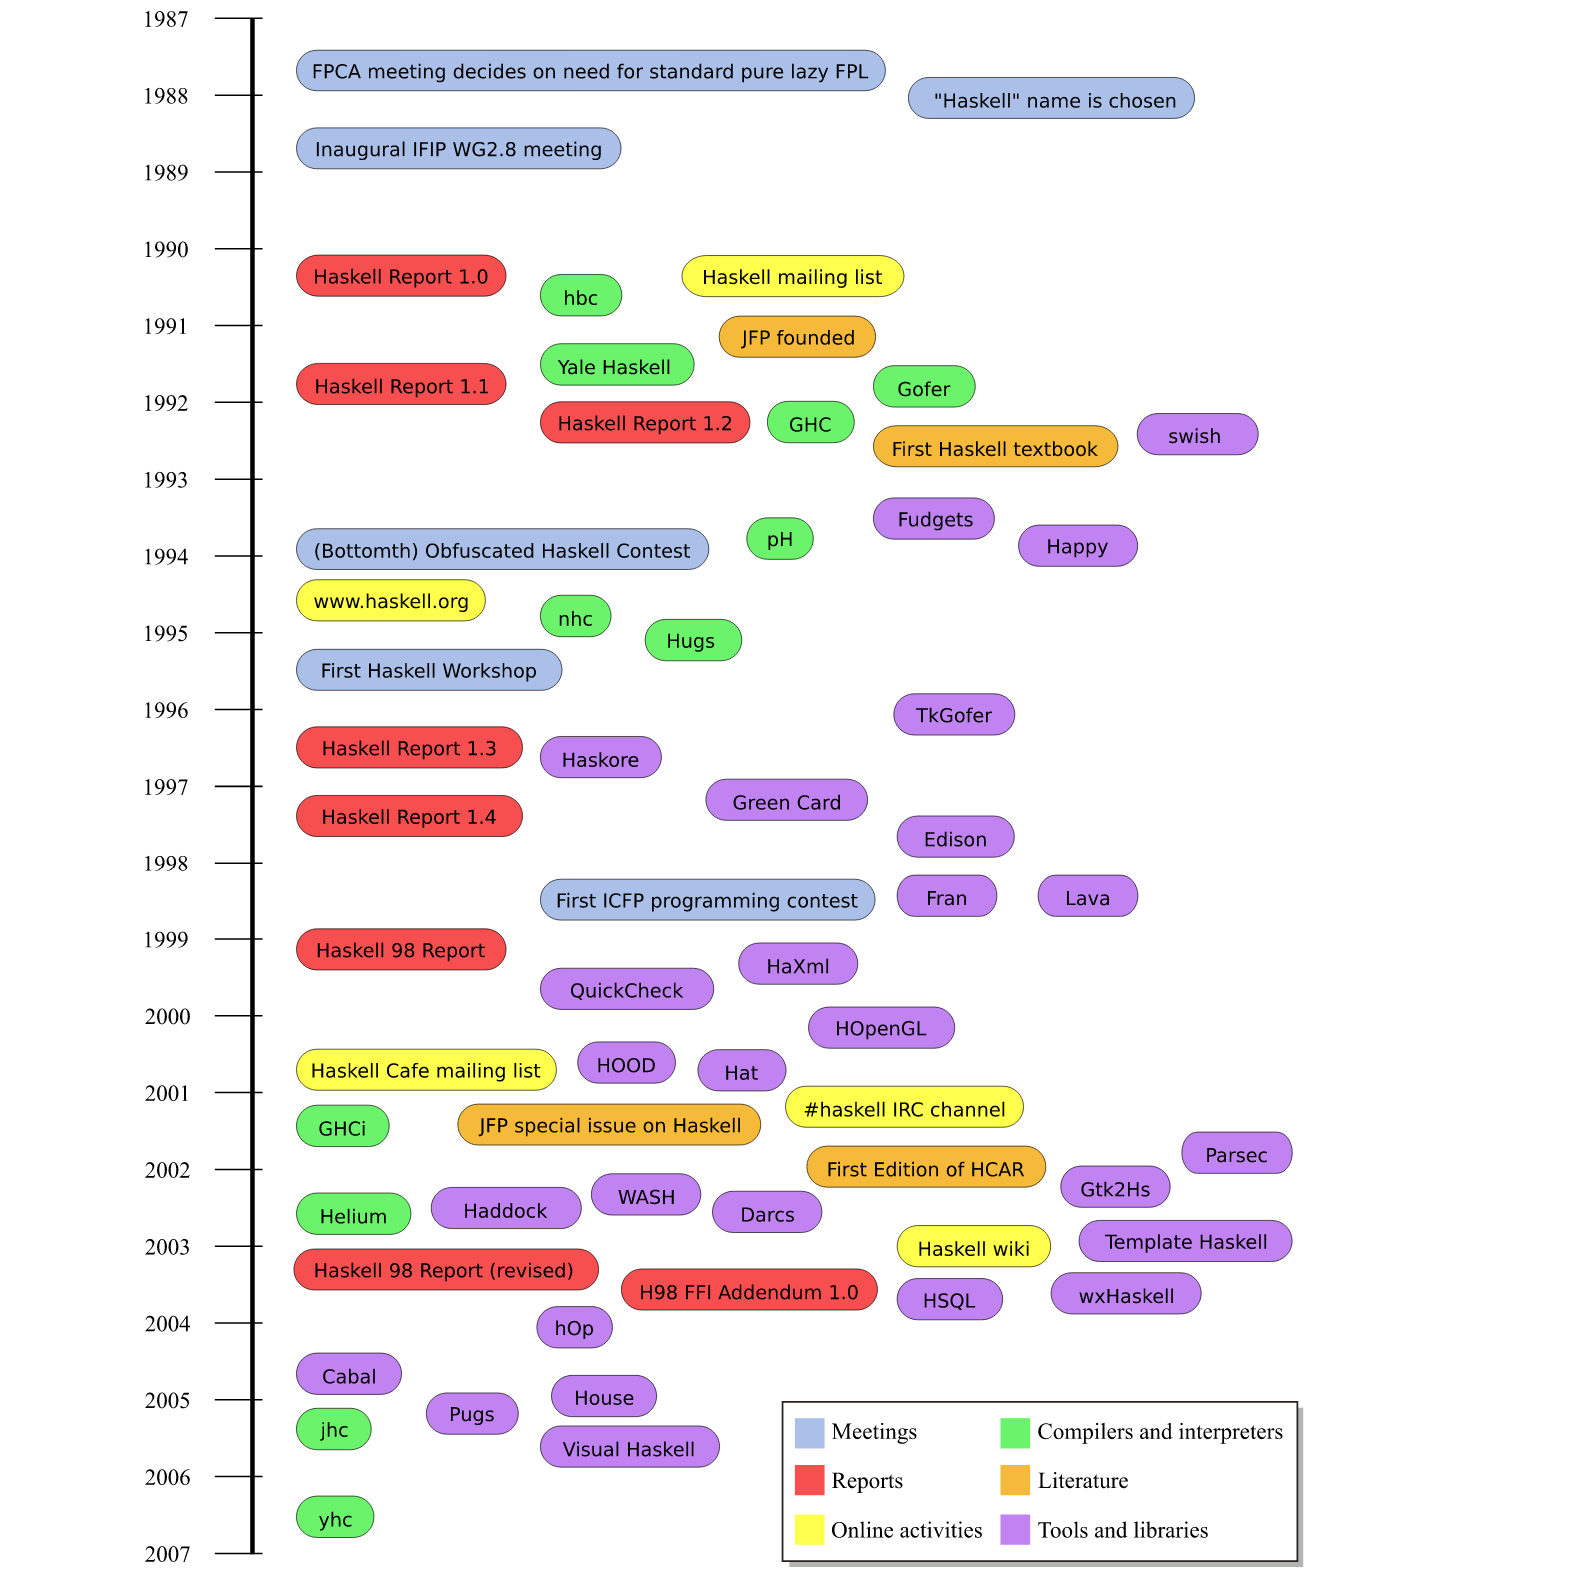
\includegraphics[width =\textwidth]{timeline.png}
      \caption{Cronologia do Haskell}
    \end{figure}

    

    \newpage

    \chapter{Paradigma a que pertence}

    O paradigma oferece e determina a visão que o programador possui sobre a estruturação
    e a execução do programa. Um exemplo bem famoso de paradigma é o POO (Programação orientada a objetos),
    conhecido por ser o modelo para linguagens como C++ e Java.

    Já a Programação funcional é um paradigma que descreve uma expressão matemática a ser avaliada,
    mapeando dos valores de entradas nos valores de retorno, por meio de funções. Em outras palavras: 
    a programação funcional só funciona em cima de funções.

    Eis mais algumas características do paradigma

    \section{Dados imutáveis} 

    É possível declarar valores a variáveis, mas não pode mudar o valor dessas 
    delas durante a compilação. Isso acontece porque, diferente de linguagens imperativas(Como C), onde você
    atribui um valor e pode mudá-lo em execuções, variáveis em Haskell(por exemplo) possuem tipagem forte, logo 
    não sofrem efeitos colaterais(\emph{side effects}).

    \section{Funções puras}

    Também presentes em linguagens como JavaScript e Python, Funções puras são aquelas que recebem 
    um parâmetro \'input\' e sempre vão retornar o mesmo \'input\' sem causar efeitos colatreis
    ao programa.

    Este tipo de função é muito boa pelos seguintes aspectos
    
    \begin{itemize}
      \item facilita execução de códigos em paralelo, pois não impactam outras funcionalidades que estão em atuação
      \item Maior facilidade em criar cache, já que os mesmos parâmetros são sempre esperados.
    \end{itemize} 

    \newpage

    \section{Cálculo Lambda}
    
    Como mencionado anteriormente, o Cálculo Lambda está presente na programação funcional, e em Haskell não é diferente.
    Em Haskell, é possível utilizar as chamadas \emph{Expressões lambda} que são funções anônimas(sem nome), formadas por 
    uma sequência de padrões:

    \begin{itemize}
      \item Argumentos da função 
      \item Corpo
    \end{itemize}

    \begin{gather*}
      \text{Função anônima para calcular o dobro de x} \\ x \rightarrow x + x 
    \end{gather*}

    \section{Análise crítica} 

    As linguas que seguem o paradigma funcional se caracterizam em criar 
    funcionalidade dentro de estruturas de fácil compreensão e definição. Isso ajuda a manter 
    a fiabilidade, e leitura do código, principalmente quando integrado a forte tipagem. Além disso,
    táis códigos se caracterizam pelo alto nível de abstração, principalmente ao utilizar as funções,
    já que isso permite supressão de detalhes da programação, e garante uma menor probabilidade 
    de erros.

    Em contraste, tais ideias podem se tornarem complicadas, quando utilizadas dentro de contextos
    onde é necessário de muitas variáveis(Exemplo: Banco de Dados). Além disso, por conta que as funções 
    possuem a característica de serem recursivas por padrão, elas tendem a ser mais ineficientes no sentido
    computacionalmente, quando comparado as linguagens imperativas. Ainda nesse ponto, funções recursivas podem gerar maior uso de memória.

    \newpage

    \chapter{Características mais marcantes da linguagem}

    \begin{itemize}
      \item Como dito anteriormente, a linguagem só faz utilização de funções e funções dentro de funções. Por isso
      Haskell é descrito como puramente funcional.
      \item Haskell possui uma sintaxe simples, elegante e concisa. Como resultado, programas em Haskell possuem 
      poucas linhas. 
      \item Além disso, a linguagem usa avaliação preguiçosa(Lazy evaluation), que é uma técnica para atrasar a computação 
      até um ponto em que o resultado da computação é considerado necessário.
      \item Tipagem estática: Verificação dos tipos usados em dados e variáveis para 
      garantir que sempre está sendo usado um tipo que é esperado em todas as situações. 
      \item função de ordem superior: Função que tem como argumento uma outra função, ou que produz 
      uma função como resultado.
    \end{itemize}

    \newpage

    \chapter{Linguagem similares ou confrontantes}

    \begin{itemize}
      \item Prolog
      \item LISP 
      \item Scheme 
      \item ML 
      \item Miranda 
      \item Elixir 
    \end{itemize}

    \newpage

    \chapter{Exemplo(s) de programa(s)}

      \setcounter{section}{0}

      \section{Hello World em Haskell}
      \lstinputlisting[language=haskell]{helloworld.hs}

      \section{Quicksort}
      \subsection{Exemplo de Quicksort em C}

      \lstinputlisting[language=c]{quicksort.c}
      \subsection{Exemplo de Quicksort em Haskell usando compreensão de lista} 

      \lstinputlisting[language=haskell]{quicksort_list.hs}      

      \newpage

      \subsection{Exemplo de Quicksort em Haskell usando a função filter}

      \lstinputlisting[language=haskell]{quicksort_filter.hs}

      \section{Explicação dos algoritmos}
      Os algoritmos em Haskell são extremamente compactos em relação à C. Sua sintaxe não tem foco
      em programar diretamente a memória, como acontece em C. Começando pelo \emph{Hello World} simples que possui ou evoluindo
      para um quicksort, a lingua mostra-se bem compacta e direta na resolução do problema.

      No primeiro exemplo, foi usado \emph{list comprehension} para resolver o problema. Na primeira linha,
      foi declarado uma lista vazia, mas poderia ser uma lista contendo quaisquer valores. A segunda linha
      cria uma função recursiva e 

      \subsection{Exemplo de Quicksort em Haskell usando a função filter}

      \lstinputlisting[language=haskell]{quicksort_c2haskell.hs}

      \newpage

      \subsection{Exemplo de Quicksort em Haskell usando a função filter} 

      \lstinputlisting[language=haskell]{quicksort_c2Haskellresumido.hs}

    \newpage

    \phantompart

    \chapter*[Considerações finais]{Considerações finais}
    \addcontentsline{toc}{chapter}{Considerações finais}

    \newpage

    \postextual

    \bibliography{abntex2-modelo-references}
    \begin{apendicesenv}
      
        \partapendices

        %Corrigir erro da numeração dos apendices
        \setcounter{chapter}{0}
        \renewcommand{\thechapter}{\Alph{chapter}}%

        \chapter{Gustavo Lopes}

        O que eu achei de Haskell? Como um usuário de longa data de linguagens orientadas a objeto(OOP), 
        como Java, C++ e mais recentemente Dart, minha experiência inicial com Haskell foi...
        um pouco estranha. Fiquei muito curioso e até encucado em ver Haskell executar códigos, que em
        outras linguagens precisariam ocupar 50 linhas, em apenas 2 ou 3 linhas, como foi o Quicksort.

        Além disso, lendo sua história, achei extremamente fascinante toda a concepção do Haskell,
        mas fiquei até triste, vendo que é muito difícil encontrar muitas pessoas falando sobre essa linguagem, que nasceu 
        do esforço coletivo de vários programadores, mas que hoje não recebe tanto apoio como outras linguagens.

        Por fim, como curiosidade, eu estava procurando sobre como fazer interfaces em C++ quando
        descobri que a WxWidgets, uma biblioteca para criar interface cross-platform , também possui 
        sua versão para Haskell, chamada WxHaskell.

        \begin{figure}[ht]
          \includegraphics[width =\textwidth]{gebob.png}
          \caption{GeBoP, um jogo de tabuleiro feito em Haskell, usando WxHaskell}
        \end{figure}

        \newpage
        
        \chapter{Thiago Henriques}

        \newpage 

        \chapter{Lucas Santiago}

        \newpage

        \chapter{Pedro Souza}




    
    \end{apendicesenv}


    \phantompart

    \printindex

\end{document}


